\documentclass{beamer}
\usepackage[utf8]{inputenc}

\usetheme{Madrid}
\usecolortheme{default}
\usepackage{amsmath,amssymb,amsfonts,amsthm}
\usepackage{txfonts}
\usepackage{tkz-euclide}
\usepackage{listings}
\usepackage{adjustbox}
\usepackage{array}
\usepackage{tabularx}
\usepackage{gvv}
\usepackage{lmodern}
\usepackage{circuitikz}
\usepackage{tikz}
\usepackage{graphicx}

\setbeamertemplate{page number in head/foot}[totalframenumber]

\usepackage{tcolorbox}
\tcbuselibrary{minted,breakable,xparse,skins}



\definecolor{bg}{gray}{0.95}
\DeclareTCBListing{mintedbox}{O{}m!O{}}{%
  breakable=true,
  listing engine=minted,
  listing only,
  minted language=#2,
  minted style=default,
  minted options={%
    linenos,
    gobble=0,
    breaklines=true,
    breakafter=,,
    fontsize=\small,
    numbersep=8pt,
    #1},
  boxsep=0pt,
  left skip=0pt,
  right skip=0pt,
  left=25pt,
  right=0pt,
  top=3pt,
  bottom=3pt,
  arc=5pt,
  leftrule=0pt,
  rightrule=0pt,
  bottomrule=2pt,
  toprule=2pt,
  colback=bg,
  colframe=orange!70,
  enhanced,
  overlay={%
    \begin{tcbclipinterior}
    \fill[orange!20!white] (frame.south west) rectangle ([xshift=20pt]frame.north west);
    \end{tcbclipinterior}},
  #3,
}
\lstset{
    language=C,
    basicstyle=\ttfamily\small,
    keywordstyle=\color{blue},
    stringstyle=\color{orange},
    commentstyle=\color{green!60!black},
    numbers=left,
    numberstyle=\tiny\color{gray},
    breaklines=true,
    showstringspaces=false,
}
%------------------------------------------------------------
%This block of code defines the information to appear in the
%Title page
\title %optional
{1.9.2}
\date{August 27,2025}
%\subtitle{A short story}

\author % (optional)
{Bhargav - EE25BTECH11013}



\begin{document}


\frame{\titlepage}
\begin{frame}{Question}
The point on the X axis which is equidistant from \brak{-4,0} and \brak{10,0} is\\ 
\end{frame}



\begin{frame}{Theoretical Solution}

Let the 2 points be $\vec{A}$ and $\vec{B}$ and let the desired point equidistant from both $\vec{A}$ and $\vec{B}$ be $\vec{O}$:
\begin{align}
    \vec{A}=\begin{myvec}{-4\\0}\end{myvec} \;, \vec{B}=\begin{myvec}{10\\0} \end{myvec}
\end{align}
\begin{align}
\vec{O} = x\,\mathbf e_1= \myvec{$x$ \\ $0$} \\
\end{align}
If $\vec{O}$ lies on $X$ axis and is equidistant from $\vec{A}$ and $\vec{B}$ \\


\end{frame}

\begin{frame}{Theoretical Solution}
\begin{align}
\|\vec{O}-\vec{A}\|=\|\vec{O}-\vec{B}\|
\end{align}

\begin{align}
\implies \|\vec{O}-\vec{A}\|^2 = \|\vec{O}-\vec{B}\|^2
\end{align}

\begin{align}
\implies (\vec{O}-\vec{A})^{\top}(\vec{O}-\vec{A}) = (\vec{O}-\vec{B})^{\top}(\vec{O}-\vec{B})
\end{align}

\begin{align}
\implies \vec{O}^{\top}\vec{O} - 2\vec{O}^{\top}\vec{A} + \vec{A}^{\top}\vec{A}
= \vec{O}^{\top}\vec{O} - 2\vec{O}^{\top}\vec{B} + \vec{B}^{\top}\vec{B}
\end{align}

\end{frame}
\begin{frame}{Theoretical Solution}

\begin{align}
\implies \|\vec{O}\|^2 - 2\vec{O}^{\top}\vec{A} + \|\vec{A}\|^2
= \|\vec{O}\|^2 - 2\vec{O}^{\top}\vec{B} + \|\vec{B}\|^2
\end{align}
\begin{align}
    (\vec{A}-\vec{B})^{\top}\vec{O}=\frac{\|\vec{A}\|^2-\|\vec{B}\|^2}{2}.
\end{align}

\begin{align}
     \vec{O} = x \mathbf{e}_1,
\end{align}

\begin{align}
    x = \frac{\|\vec{A}\|^2 - \|\vec{B}\|^2}{2 (\vec{A} - \vec{B})^{\top} \mathbf{e}_1}.
\end{align}

Solving for $x$, we get $x$ = $3$\\

\begin{align}
    \therefore \vec{O} = \myvec{$3$ \\ $0$}
\end{align}
\end{frame}

\begin{frame}[fragile]
    \frametitle{C Code - Equidistant point}

    \begin{lstlisting}

#include <stdio.h>
#include <math.h>

// Function to compute x-coordinate of equidistant point
double equidistant_point(double ax, double ay, double bx, double by) {
    // Norm squared of A and B
    double normA2 = ax*ax + ay*ay;
    double normB2 = bx*bx + by*by;

    double denom = 2 * (ax - bx);

    
    double x = (normA2 - normB2) / denom;
    return x;
}



    \end{lstlisting}
\end{frame}

\begin{frame}[fragile]
    \frametitle{Python + C Code}
    \begin{lstlisting}
import ctypes
import numpy as np
import matplotlib.pyplot as plt

# Load the C shared library
lib = ctypes.CDLL("./libequidistant.so")

# Define function prototype: double f(double, double, double, double)
lib.equidistant_point.argtypes = [ctypes.c_double, ctypes.c_double,
                                  ctypes.c_double, ctypes.c_double]
lib.equidistant_point.restype = ctypes.c_double

# Define A and B
A = np.array([-4.0, 0.0])
B = np.array([10.0, 0.0])




    \end{lstlisting}
\end{frame}

\begin{frame}[fragile]
    \frametitle{Python + C Code}
    \begin{lstlisting}
# Call C function
x = lib.equidistant_point(A[0], A[1], B[0], B[1])

# Equidistant point
O = np.array([x, 0.0])

print("Equidistant point O =", O)

# ---- Plotting ----
plt.figure(figsize=(6,6))
plt.axhline(0, color='gray', linewidth=0.8)
plt.axvline(0, color='gray', linewidth=0.8)

# Plot points
plt.scatter(A[0], A[1], color='red', label='A (-4,0)')
plt.scatter(B[0], B[1], color='blue', label='B (10,0)')
plt.scatter(O[0], O[1], color='green', marker='*', s=150, label=f'O ({int(O[0])},0)')




    \end{lstlisting}
\end{frame}

\begin{frame}[fragile]
    \frametitle{Python + C Code}
    \begin{lstlisting}
# Connect O to A and B
plt.plot([A[0], O[0]], [A[1], O[1]], 'r--')
plt.plot([B[0], O[0]], [B[1], O[1]], 'b--')

plt.legend(loc="upper right")
plt.grid(True, linestyle='--', alpha=0.6)
plt.title("Equidistant Point on X-axis (C + Python)")
plt.xlabel("x")
plt.ylabel("y")
plt.axis("equal")
plt.savefig("/Users/bhargavkrish/Documents/ee1030-2025/ee25btech11013/matgeo/1.9.2/figs/Figure_1.png")
plt.show()

    \end{lstlisting}
\end{frame}



\begin{frame}[fragile]
    \frametitle{Python Code}
    \begin{lstlisting}
import numpy as np
import matplotlib.pyplot as plt


A = np.array([-4, 0])
B = np.array([10, 0])


e1 = np.array([1, 0])


num = np.linalg.norm(A)**2 - np.linalg.norm(B)**2
den = 2 * np.dot(A - B, e1)
x = num / den


O = x * e1


    \end{lstlisting}
\end{frame}

\begin{frame}[fragile]
    \frametitle{Python Code}
    \begin{lstlisting}

print("Point equidistant from A and B on x-axis:", O)


plt.figure(figsize=(6,6))
plt.axhline(0, color='gray', linewidth=0.8)  # x-axis
plt.axvline(0, color='gray', linewidth=0.8)  # y-axis

# Plot points
plt.scatter(A[0], A[1], color='red', label='A (-4,0)')
plt.scatter(B[0], B[1], color='blue', label='B (10,0)')
plt.scatter(O[0], O[1], color='green', marker='*', s=150, label=f'O ({int(O[0])},0)')


plt.plot([A[0], O[0]], [A[1], O[1]], 'r--', linewidth=1)
plt.plot([B[0], O[0]], [B[1], O[1]], 'b--', linewidth=1)




    \end{lstlisting}
\end{frame}

\begin{frame}[fragile]
    \frametitle{Python Code}
    \begin{lstlisting}
plt.legend(loc="upper right")
plt.grid(True, linestyle='--', alpha=0.6)
plt.title("Equidistant Point on X-axis")
plt.xlabel("x")
plt.ylabel("y")
plt.axis("equal")
plt.savefig("/Users/bhargavkrish/Documents/ee1030-2025/ee25btech11013/matgeo/1.9.2/figs/Figure_1.png")
plt.show()
    \end{lstlisting}
\end{frame}

\begin{frame}{Plot}
    \centering
    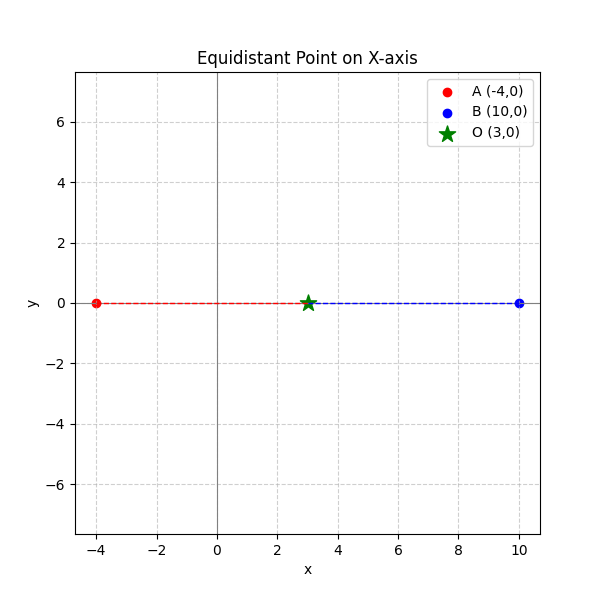
\includegraphics[width=3\columnwidth, height=0.8\textheight, keepaspectratio]{figs/Figure_1.png}     
\end{frame}


\end{document}